\documentclass[12pt]{article}

\usepackage[paperheight=1.5in,paperwidth=4in,top=.25in,bottom=0in,right=0in,left=0in]{geometry}
%fancy math symbols
\usepackage{amsmath}
\usepackage{amssymb}
\usepackage{cancel}
%fancy font
%\usepackage{pxfonts}
\usepackage[T1]{fontenc}
%DAGs
\usepackage{tikz}
\usetikzlibrary{arrows,positioning,snakes,calc,shapes}
\tikzset{>=latex}
\usepackage{subfig}
\captionsetup[subfloat]{position = top, font = large} % For sub-figure captions
\renewcommand{\thesubfigure}{\normalsize\Alph{subfigure})}
\usepackage{float}

\begin{document}
\begin{figure}[H] %\rule{\textwidth}{1pt} 
\begin{center}\large
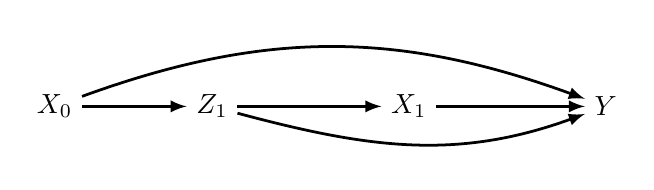
\begin{tikzpicture}
\node[align = center] (x0) at (0,1) {$X_{0}$};
\node[align = center] (z) at (2,1) {$Z_{1}$};
\node[align = center] (x1) at (4.5,1) {$X_{1}$};
\node[align = center] (y) at (7,1) {$Y$};
\begin{scope}[line width = 1pt]
\draw[->,color=black] (x0) to (z);
\draw[->,color=black] (z) to (x1);
\draw[->,color=black] (x1) to (y);
\draw[->] (x0) to [out=20,in=160] (y);
\draw[->] (z) to [out=345,in=200] (y);
\end{scope}
%\draw[help lines] (0,0) grid (7,2) ;
\end{tikzpicture}
\end{center}
\end{figure}
\end{document}